%----------------------------------------------------------------------------------------
%	PACKAGES AND THEMES
%----------------------------------------------------------------------------------------
\documentclass[aspectratio=169,xcolor=dvipsnames]{beamer}
\usetheme{SimplePlus}

\usepackage{hyperref}
\usepackage{graphicx} % Allows including images
\usepackage{booktabs} % Allows the use of \toprule, \midrule and \bottomrule in tables

%----------------------------------------------------------------------------------------
%	TITLE PAGE
%----------------------------------------------------------------------------------------

\title[short title]{On Local Optima Distribution in Buffer Allocation Problem for Production Line with Unreliable Machines} % The short title appears at the bottom of every slide, the full title is only on the title page
%\subtitle{Subtitle}

\author[authors]{ Alexandre Dolgui$^1$, Anton Eremeev$^2$, Viatcheslav Sigaev$^3$} 


\institute[NTU] 
{
    $^1$IMT Atlantique, Nantes, France \\
    $^2$Sobolev Institute of Mathematics SB RAS, Novosibirsk \\
    $^3$Avtomatika-Servis LLC, Omsk
}
\date{\today} % Date, can be changed to a custom date


%----------------------------------------------------------------------------------------
%	PRESENTATION SLIDES
%----------------------------------------------------------------------------------------

\begin{document}

\begin{frame}
    % Print the title page as the first slide
    \titlepage
\end{frame}

\begin{frame}{Overview}
    % Throughout your presentation, if you choose to use \section{} and \subsection{} commands, these will automatically be printed on this slide as an overview of your presentation
    \tableofcontents
\end{frame}

%------------------------------------------------
\section{Buffer Allocation Problem}
%------------------------------------------------

\begin{frame}{Buffer Allocation Problem}
\vspace{-0.5cm}	
\begin{columns}
 \column{.65\textwidth}
    \begin{figure}
    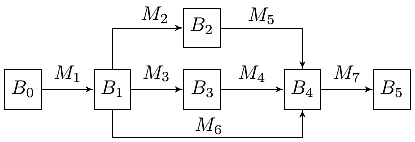
\includegraphics[scale=0.9]{LineSchems}
    \end{figure}
 \column{.45\textwidth}    
	Parameters of machine $M_i$:
     \begin{itemize}
	\item $\lambda_i$ is the failure rate;
	\item $\mu_i$ is  the repair rate;
	\item $u_i$ is the average production rate.
    \end{itemize}
\end{columns}    
\vspace{0.5cm}	
    \begin{itemize}
	\item Machines may break down only when they are working.
	\item The time to failure and time to repair for each machine are mutually independent and exponentially distributed.
	\item Working machine has a constant cycle time and production rate.
	\item There is a sufficient number of raw parts at the input of the system.
	\item The completed parts depart from the system immediately.
    \end{itemize}
\end{frame}

%------------------------------------------------

\begin{frame}{Performance Evaluation Methods}
    \begin{itemize}
	\item Existence of steady-state distribution + asymptotic analysis\\
	(Sevast'yanov B. A.,1962)
	\item Differential Kolmogorov equations for two michines and buffer between them \\
	(Levin A.A. \& Pasko N.I.,1969).
	\item Integral equations for serial lines of two and three machines and buffers between them\\
	(Coillard P. \& Proth J. M,1984).
	\item Aggregation and decomposition techniques for evaluation of multiple-machine tandem lines\\
	(Gershwin et al.,1987, 1994, 2009),(Dallery Y., David R., Xie X., 1988)\\
	(Dolgui \& Svirin, 1992)\\
    \end{itemize}
    \begin{figure}
    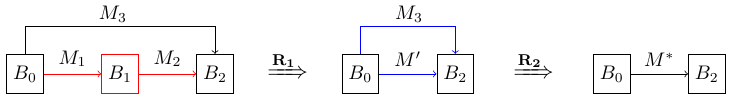
\includegraphics[scale=0.8]{alg_line}
    \end{figure}
\end{frame}

%------------------------------------------------

\begin{frame}{Optimization criterion}
\begin{equation}
\max \varphi(H)=T_{am} R(V(H)) - Q(H) - J(H),
\end{equation}
where 
\begin{itemize}
\item $T_{am}$  is the amortization time of the line (line life); 
\item $V(H)$ is the average production rate (steady state throughput); 
\item $R(V)$  is the revenue related to the production rate $V$; 
\item $J(H)$ is the cost of buffer configuration $H$; 
\item $d_j$ is the maximal admissible capacity of buffer $B_j$;
\item $Q(H)= c_1q_1(H)+ …+c_n q_n(H)$ is the average steady state inventory cost, where $q_j(H)$ is the average steady state number of parts in buffer $b_j$, for $j=1,…,n$.
\end{itemize}
    \begin{block}{NP~hard}
       The buffer allocation problem is known to be NP~hard as shown by Dolgui et al. (2013)
    \end{block}
\end{frame}

%------------------------------------------------

\begin{frame}{Problem Instances}
\begin{table}[!ht]
\centering
\small
\begin{tabular}{|c|c|c|}
\hline
 \textbf{Series}& \textbf{Number of Lines}& \textbf{Number of Machines}\\
\hline
AS & 8 & 4 -- 14 \\
BN & 10 & 5 \\
VP & 4 & 5 \\
\hline
\end{tabular}
\caption{List of series}\label{tabl:series}
\end{table}
\vspace{-0.2cm}	
 \begin{figure}[h!]
	\centering
	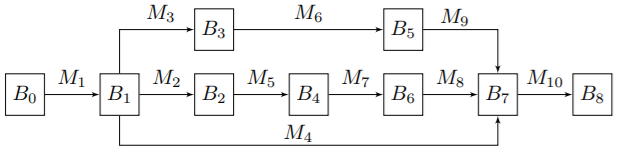
\includegraphics[scale=0.6]{ans7}
\vspace{-0.3cm}	
  \caption{Line structure AS7} \label{fig:vis_as7}
  \end{figure}
\vspace{-0.2cm}	
 \begin{figure}[h!]
	\centering
	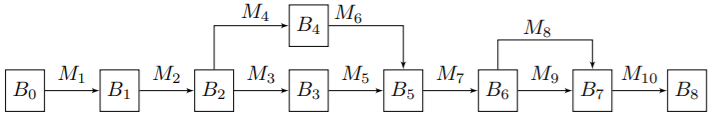
\includegraphics[scale=0.55]{ans8}
	\vspace{-0.3cm}
  \caption{Line structure AS8} \label{fig:vis_as8}
  \end{figure}
\end{frame}

%------------------------------------------------
\section{Alghoritms}
%------------------------------------------------

\begin{frame}{Local search algorithms}
\begin{itemize}
\item \textbf{Local search algorithm (LSA)}. At each iteration, the LSA searches through the neighborhood of radius 1 in metric $l_1$ around
the current solution. If an improving feasible solution in terms of the  objective function is found in the neighborhood, then it becomes the new current solution.
\vspace{1cm}
\item \textbf{Tabu-search algorithm (TS)} is a metaheuristic search method  that uses local search procedure and rejects moves to points already visited in the search space by means of the so-called tabu list.
\end{itemize}
\end{frame}

%------------------------------------------------
<<<<<<< HEAD
\section{''Big Valley'' or ''Massif Central''}
=======

\begin{frame}{Genetic algorithms}
    \begin{figure}
    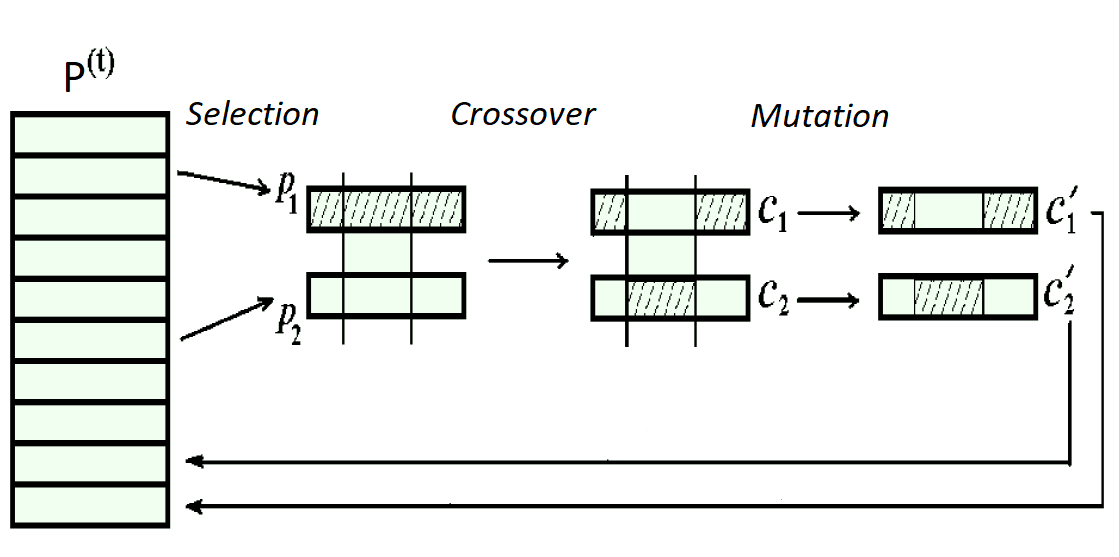
\includegraphics[scale=0.4]{schGA}
    \end{figure}
\begin{itemize}
\item \textbf{Genetic algorithm (pure GA)} is a metaheuristic that is based on natural selection, the process that drives biological evolution.
\item \textbf{Genetic algorithm with LSA (GA)} is pure GA which improved by using LSA after mutation.
\end{itemize}
    
\end{frame}

%------------------------------------------------
\section{Hypothesis ''Big Valley'' or ''Massif Central''}

\begin{frame}{Hypothesis ''Big Valley'' or ''Massif Central''  (Boese et al.
1993)}
\begin{enumerate}
\item Values of the objective function in the local optima tend to deteriorate with increasing distance to the global optimum (i.e. there is a correlation 
of objective function in the local optima with the distance to the global optimum).
\vspace{0.5cm}	
\item Local optima are located relatively close both to each other and to the global optimum (they are located in a ball, which is smaller than 
the whole search space by several orders of magnitude).
\end{enumerate}

{\bf Let }
\begin{itemize}
\item $V1$ be the cardinality of the intersection of feasible solutions with the ball (in the norm~$\ell_1$) containing
all local optima, and 
\item $V2$ denote the cardinality of the entire set of feasible
solutions.
\end{itemize}
\end{frame}

%------------------------------------------------

\begin{frame}{Ratio $V1/V2$ for all series}
    \begin{figure}
    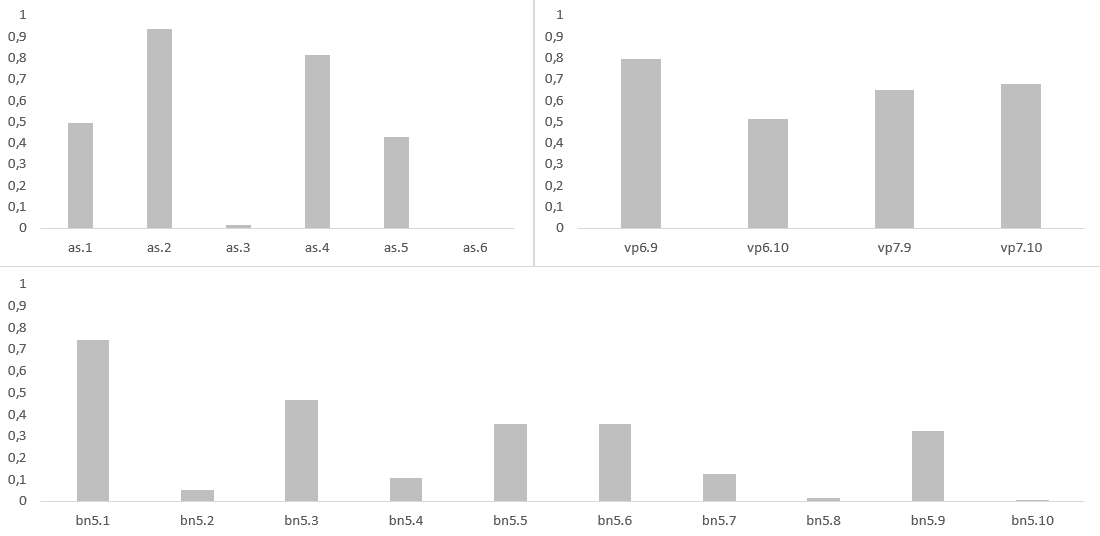
\includegraphics[scale=0.6]{volume}
    \end{figure}
\end{frame}

%------------------------------------------------

\begin{frame}{Negated correlation $-\rho(r(\xi, \xi*),\varphi(\xi))$ for all series}
    \begin{figure}
    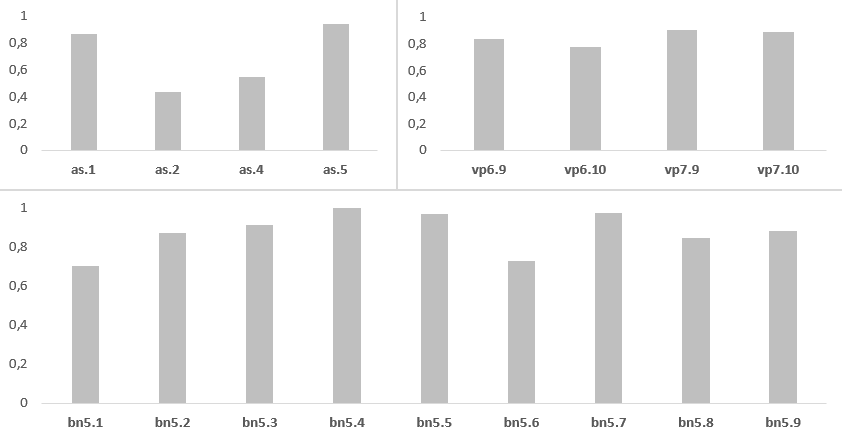
\includegraphics[scale=0.8]{ro}
    \end{figure}
\end{frame}

%------------------------------------------------
\section{Clustering effect}
%------------------------------------------------

\begin{frame}{Clustering effect of local optima}
\begin{columns}
 \column{.5\textwidth}
 \begin{figure}
	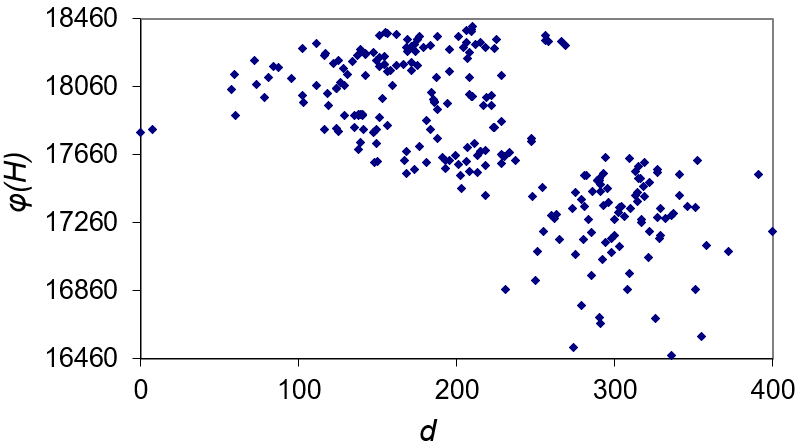
\includegraphics[scale=0.4]{multistart_klaster}
	\caption{The set of local optima obtaained in as.4 } 	
  \end{figure}
 \column{.5\textwidth}  
   \begin{figure}
	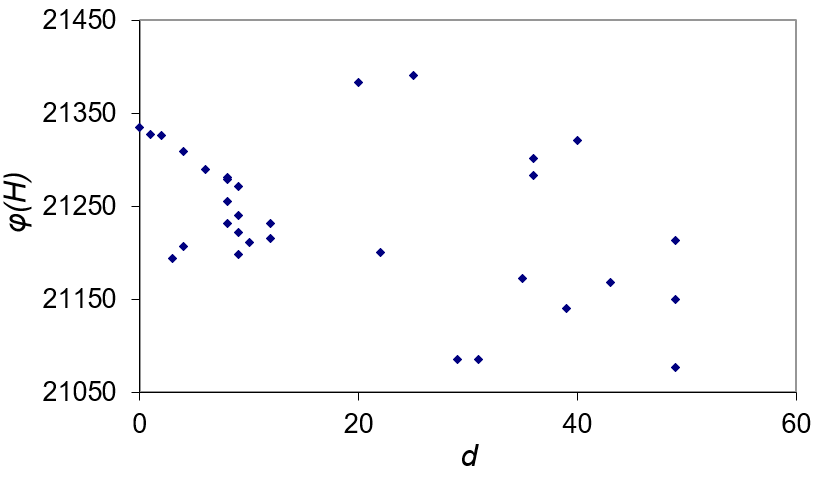
\includegraphics[scale=0.4]{klaster_bn5_1.png}
	\caption{The set of  local optima obtained in bn5.1.} 
  \end{figure}
 \end{columns}  
\end{frame}

%------------------------------------------------

\begin{frame}{Clustering effect reasons}
\begin{columns}
 \column{.65\textwidth}
    \begin{block}{Parallel sections in line}
        If there are two parallel paths that are identical in their network structure,
such that one path will have relatively large buffers, and other one will have relatively small buffers, then 
it is possible to obtain two solutions with close values of the objective function, but located at a large distance from each other.
    \end{block}
 \column{.35\textwidth}
     \begin{figure}
    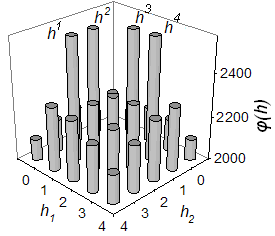
\includegraphics[scale=0.6]{test}
    \end{figure}
 \end{columns}
    \begin{block}{Two-machine line symmetry}
        This property is indicated by  by Levin and Pasjko
(1969) for a serial line,
consisting of two machines and a buffer
between them. If we swap the parameters of the first and the second machines so 
that the input buffer of the line will become its output, and the output buffer will become the input, then
line performance will not change.
    \end{block}
   
\end{frame}

%-----------------------------------------------
\begin{frame}{Cluster structure of GA population of as.4 problem}
    \vspace{-0.5cm}
    \begin{figure}
    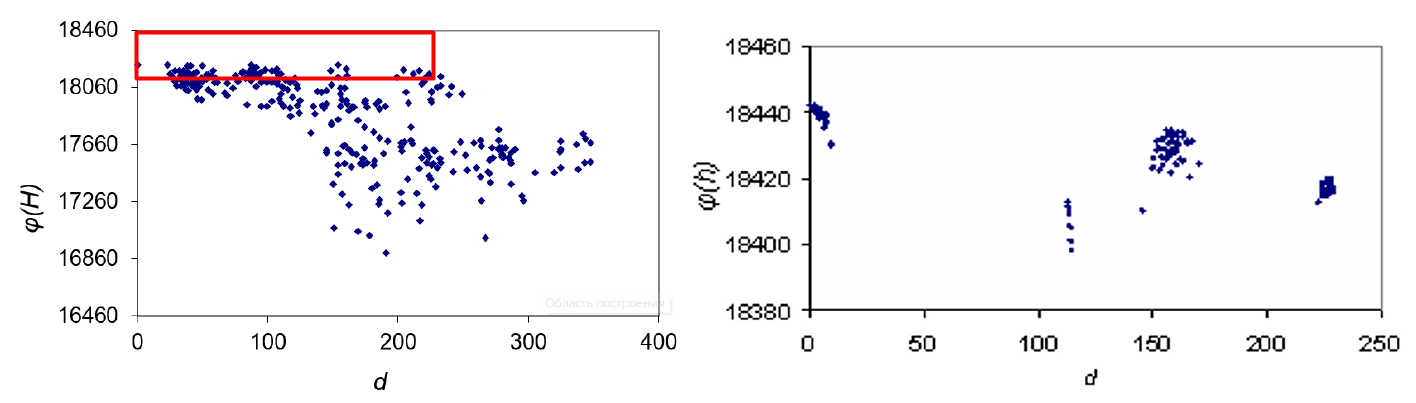
\includegraphics[scale=0.5]{ga_klasters}
    \end{figure}
        \begin{block}{Cluster structure}
 The experiments have shown, the population of the pure GA, and that of the GA with local search, contain individuals from different clusters.
    \end{block}
\end{frame}

%------------------------------------------------
\section{Future research}
%------------------------------------------------

\begin{frame}{Future research}
        \begin{block}{Improving GA}
The GA could be further improved if each pair of parent solutions were chosen from the same cluster (then the crossover could have a similar effect as e.g. in Dang et al. (2016)).
    \end{block}
    \vspace{1cm}	
            \begin{block}{Excluding the equivalent solutions}
Excluding the equivalent solutions in view of the problem symmetries may 
reduce the number of clusters in the GA population.    
    \end{block}
 \end{frame}

%------------------------------------------------

\begin{frame}
    \Huge{\centerline{\textbf{The End}}}
\end{frame}

%----------------------------------------------------------------------------------------

\end{document}